\documentclass[conference]{IEEEtran}
\usepackage{iftex}
\ifXeTeX
  \usepackage{fontspec}
  \setmainfont{texgyretermes}[Extension=.otf,UprightFont=*-regular,BoldFont=*-bold,ItalicFont=*-italic,BoldItalicFont=*-bolditalic]
\fi
\usepackage{graphicx}
\usepackage{amsmath}
\usepackage{booktabs}
\usepackage{url}
\usepackage[hidelinks]{hyperref}

\begin{document}

\title{Predict the Breach, Not the Drop:\\Control-Aligned Learning for Smoothing\\AI Training Power Swings}

\author{\IEEEauthorblockN{Sayed Raheel Hussain}
\IEEEauthorblockA{Kayaan AI, New York, NY, USA\\
\texttt{sayed@kayaan.ai}}}

\maketitle

\begin{abstract}
AI training jobs swing GPU power by tens of percent within a second, creating fast load ramps at
grid-connected facilities. In an idealized simulation, fill-type smoothing reduces ramp-threshold
violations but must be engaged before the fall, at a cost. The forecasting target matters. In a
matched-pipeline ablation, a gradient-boosted classifier trained on the usual target, a large power drop,
ranks violations poorly (average precision 0.58). Trained on the controller's own event,
a violation inside the window a limiter armed now would cover, it reaches 0.96 on
held-out H100 traces, against 0.67 for rhythm replay. With a validation-chosen threshold, the
learned trigger removes 86.8\% of test violations while engaged
45.6\% of the time; rhythm replay must stay engaged 99.2\%.
Across three public datasets, learning significantly beats rhythm replay on two when the site is in the
training data. Transfer to unseen sites is unreliable.
\end{abstract}

\begin{IEEEkeywords}
Data centers, energy storage, load forecasting, machine learning, power smoothing
\end{IEEEkeywords}

\section{Introduction}
Training a large model alternates compute-heavy and communication-heavy phases, so GPU power moves in
fast, large steps. Because all nodes of a job step together, a synchronized job appears to the grid as
one large swing; industry reports describe swings of tens to hundreds of megawatts and evaluate software
power burning, GPU power floors and rack storage as mitigations~\cite{msft_stab}. Hardware filters and
storage that react to the measured load are being developed~\cite{easyrider,activefilter}; predictive
storage control has been studied with perfect preview~\cite{hessdpc} and with short delay-compensating
predictors~\cite{lyu}; and AI data center load has been forecast at minute scales~\cite{mughees}. We are
not aware of work that studies how the forecasting target affects smoothing performance.

A fill-type actuator must be engaged before the fall arrives, but engagement costs energy and readiness
(a hot inverter, pre-warmed filler kernels). A forecaster can engage the actuator only when needed. The
obvious competitor is free: training power is periodic, so ``replay the last cycle'' is a strong
predictor. Our contributions:
\begin{itemize}
\item A control-aligned prediction target: a ramp-limit violation that falls entirely inside the window
a limiter armed now would cover, instead of a generic ``large drop''.
\item A readiness analysis (violations removed versus time engaged) comparing learned triggers, rhythm
replay, an always-on limiter and a perfect-foresight oracle in one simulator.
\item A three-dataset study (H100, B200, V100; benchmarks and labelled cluster jobs) with job-clustered confidence
intervals, a sensor-harmonization step, and a negative result on unseen sites.
\end{itemize}

\section{Data}
\textbf{NLR}~\cite{nlr}: 4$\times$H100 nodes running MLPerf Llama2-70B LoRA and Stable Diffusion
training on 1--16 nodes, plus three vLLM Llama3.1-70B inference benchmarks, NVML power at 5--10~Hz,
248 node-hours (at most four nodes per job, which run nearly in lockstep, are kept; all
are weighted equally in metrics). Training jobs are split whole into train, validation and test; each
inference benchmark is a single continuous session split in time, so its test portion counts as one
independent unit. \textbf{Elsayed et al.}~\cite{elsayed}: single 8$\times$H100 and 8$\times$B200 nodes
running diffusion and Llama 1B--8B fine-tuning sweeps, 15-minute sessions, 32 unique
sessions. \textbf{MIT Supercloud}~\cite{supercloud}: a stratified subset of 560 labelled jobs (80 per
model class: VGG, ResNet, Inception, U-Net, BERT, DistilBERT, GNN) on nodes with one or two V100s,
nvidia-smi at 10~Hz, 1,292 node-hours of labelled cluster jobs.

All traces are averaged onto a 0.2~s grid and expressed as ``NLR-equivalent watts'' (power $\times$
2.8~kW divided by the node's rated GPU power), so a 10\%/s limit means the same fraction of rated power
everywhere. Jobs are assigned whole to train, validation and test (about 60/20/20). For the
control-aligned models, validation units are split into two halves, one for early stopping and one for
choosing operating points; for NLR inference the validation halves are alternate hour blocks of the
same session and so are not independent. (The big-drop baselines from earlier work were early-stopped on all
validation units.)

\textbf{Sensor harmonization.} NVML documents that on recent architectures the default power reading is
averaged over about 1~s, while older GPUs such as the V100 report instantaneous power~\cite{nvml}. The NLR
documentation does not state which reading was logged. Raw V100 traces flicker: without harmonization,
91\% of Supercloud test seconds are labelled ``violation imminent''. We apply a 1~s trailing mean to
Supercloud so that all three datasets are compared at similar effective bandwidth.

\section{Problem and methods}
\subsection{Ramp limit, limiter and readiness}
For this study, a violation starts when the node's 1~s down-ramp exceeds an illustrative threshold of
10\% of rated power per second; this is a normalized study threshold, not a specific utility requirement. A fill-type limiter adds
power only when the load falls faster than the limit allows, then tapers at 90\% of the allowed rate. A trigger
issued at row $t$ acts one sample later (each row averages $[t, t{+}0.2\,\mathrm{s})$), engages the
limiter after an actuator latency $L$ (1~s unless stated) and arms it for 6~s; the limiter keeps
filling until it meets the load. We count as \emph{engaged} every sample where the limiter is armed or
still filling, and report violations removed against engaged time. We also report an energy metric
consisting of fill energy plus an assumed standby draw of 0--5\% of rated power while engaged; for
storage, this is absorbed charge before any later discharge or loss, which the simulation does not model. References: always-on, always-burn (a floor at 80\% of the trailing 60~s peak,
which removes only 6.7\% of violations for 6.8\% extra energy) and an oracle that
arms just in time for every violation, including those induced by the limiter itself.

\subsection{Targets}
The \emph{big-drop} target labels $t$ positive if a fall of more than 30\% of the recent peak within
1~s starts in the next 5~s. The \emph{control-aligned} target labels $t$ positive if the whole 1~s ramp window
of a raw violation lies inside the 6~s window during which a trigger at $t$ keeps the limiter armed, so
the limiter is armed throughout that fall. Violations induced by the limiter itself are not labelled.
Many violations (e.g.\ the 22\% square wave of Llama LoRA training) are not big drops, so the two
targets differ substantially.

\subsection{Predictors}
\emph{Rhythm replay} estimates the period $P$ from a trailing 120~s autocorrelation, predicts
$\hat p(t+k)=p(t+k-P\lceil k/P\rceil)$, and scores the largest predicted 1~s down-ramp inside the
target window; it needs no training. The \emph{learned} predictor is LightGBM~\cite{lightgbm} on 56 trailing features
(lags, differences, rolling statistics, time since recent steps and drops, rhythm period, phase and
rhythm forecasts), one model per actuator latency. The big-drop model in the readiness comparison is an
earlier configuration with different leaf-size and early-stopping choices, so that comparison does not
isolate the label alone; the matched ablation does. A shape-only variant divides every level feature by
the trailing 60~s maximum.

\subsection{Evaluation}
Ranking quality is average precision (AP) on test rows. Uncertainty is a paired bootstrap over
independent clusters (training jobs, or inference sessions; 1000 resamples). Operating points are chosen
on the validation threshold half and scored on test. All intervals are conditional on the single fitted
model and split: they resample test clusters but do not retrain. Cross-dataset comparisons score one
decision per second; the NLR readiness analysis scores every 0.2~s row.

\section{Results}
\subsection{Training target}
On NLR test traces, rhythm replay ranks the control-aligned event with AP 0.67; LightGBM trained
on the control-aligned target reaches 0.96, and the gain holds for each workload (Table~\ref{tab:wl}).
\emph{Matched label ablation.} Training the big-drop label through the same pipeline (same rows, features,
LightGBM settings, early-stopping data and metric, and square-root class-weighting rule, which gives weight
1.75 for the aligned and 2.57 for the big-drop target) yields AP 0.58 on the aligned event
against 0.96, a paired cluster-bootstrap difference of 0.37 (95\% CI
0.28 to 0.49, 12 clusters). The big-drop model is good at its own task
(AP 0.93 on the big-drop event, where the aligned model reaches
0.48): the two labels describe different events.
Results are stable across actuator latencies (AP 0.96 at 0~s, 0.95
at 3~s; rhythm replay 0.68 and 0.67).

\begin{table}[t]
\centering
\caption{NLR test AP on the control-aligned target (1~s latency).}
\label{tab:wl}
\begin{tabular}{lcc}
\toprule
Workload & Learned & Rhythm replay\\
\midrule
Llama2-70B LoRA training & 1.00 & 0.81\\
Stable Diffusion training & 0.96 & 0.73\\
Offline inference & 0.55 & 0.29\\
Online inference, finite & 0.76 & 0.09\\
Online inference, fixed rate & 0.65 & 0.36\\
\bottomrule
\end{tabular}
\end{table}

\subsection{Readiness}
Fig.~\ref{fig:ready} sweeps each trigger's threshold (about 200 validation-score quantiles) on NLR test
traces. Every trigger can reach high removal by staying engaged long enough; what differs is the engaged
time needed (Table~\ref{tab:arm}). Table~\ref{tab:arm} reads the best threshold off each test curve, so
it is a retrospective comparison of attainable trade-offs, not a deployable operating point; the
validation-chosen operating points follow below.
To remove 90\% of violations, the control-aligned learned trigger needs 48.4\%
engaged time, whereas rhythm replay of the same target reaches 90\% only at 99.2\%,
i.e.\ it is no better than always-on. The paired cluster-bootstrap difference is
$-$50.8 points (95\% CI $-$57.4 to
$-$8.8), and $-$40.8 points at 95\% removal (CI
$-$49.1 to $-$31.4). The earlier configured big-drop trigger
needs more engaged time than the control-aligned one (64.3\% at 90\%; difference
$-$15.9 points, CI $-$25.7 to $-$3.9). At 95\%
removal the interval includes zero (CI $-$26.3 to 0.5), so with
12 test clusters and non-identical configurations, the matched ablation is the cleaner evidence for the
target's effect (AP 0.58 vs 0.96). The oracle removes all violations at 29.8\% engaged time, which bounds what
better prediction could still gain.

\begin{table}[t]
\centering
\caption{Engaged time (\% of time) needed to reach a violation-removal level, NLR test, 1~s latency.}
\label{tab:arm}
\begin{tabular}{lccc}
\toprule
Removal & Learned, aligned & Rhythm, aligned & Learned, big-drop\\
\midrule
80\% & 43.1 & 51.5 & 53.0\\
90\% & 48.4 & 99.2 & 64.3\\
95\% & 58.4 & 99.2 & 74.8\\
\bottomrule
\end{tabular}
\end{table}

\begin{figure}[t]
\centering
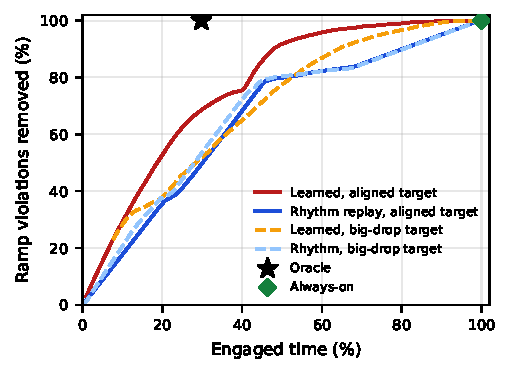
\includegraphics[width=\columnwidth]{fig_readiness.pdf}
\caption{Violations removed versus engaged time on NLR test traces (1~s latency, dense threshold sweep).
Always-on removes everything but is always engaged.}
\label{fig:ready}
\end{figure}

With operating points chosen on validation and a standby draw of 2\% of rated power, a 90\% target
gives 86.8\% removal at 45.6\% engaged time and
a 3.7\% energy metric for the learned trigger; rhythm replay meets the target only
by staying engaged 99.2\% of the time (5.4\%
energy metric, versus 5.4\% for always-on). At an 80\% target the validation-chosen
learned threshold undershoots on test (73.7\% removal), a reminder that operating
points chosen on few validation jobs transfer imperfectly.

\subsection{Across sites and GPUs}
Fig.~\ref{fig:forest} summarizes the learned-minus-rhythm AP difference. Trained on the test site's own
training jobs (in-domain) or on all three datasets (pooled), the learned trigger significantly beats
rhythm replay on NLR (pooled AP 0.96 vs 0.67) and on labelled Supercloud jobs
(pooled 0.88 vs 0.74; exploratory per-class intervals, without multiplicity correction, are
positive for 7 of 7 model classes). On Elsayed the point estimate favours learning
(0.92 vs 0.88) but the interval includes zero with six test
sessions, and rhythm replay is better on its diffusion sessions; we hypothesize that their very regular
cadence suits replay, but two test sessions do not allow a firm conclusion.

\begin{figure}[t]
\centering
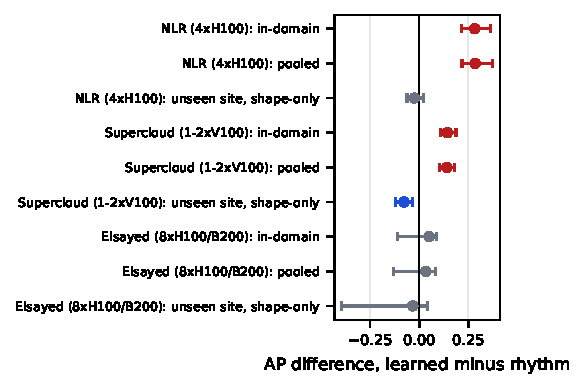
\includegraphics[width=\columnwidth]{fig_forest.pdf}
\caption{AP difference between the learned control-aligned trigger and rhythm replay, with 95\%
cluster-bootstrap intervals. Red: learned significantly better; blue: rhythm significantly better;
grey: inconclusive. Unseen-site rows use shape-only features.}
\label{fig:forest}
\end{figure}

\subsection{Unseen sites}
When the test dataset is excluded from training, the learned trigger is not better than rhythm replay
anywhere. With shape-only features it reaches AP 0.65 on NLR (rhythm
0.67, CI of difference $-$0.06 to 0.02),
0.85 on Elsayed (rhythm 0.88), and
0.66 on Supercloud, significantly below rhythm replay
(0.74; CI $-$0.12 to $-$0.04).
Continuing to train on 60 minutes of the new site's data (mean of five independent draws) gives
0.71 on NLR (range 0.62 to
0.77) and 0.64 on Supercloud (range
0.58 to 0.69), so a short
calibration period does not reliably recover the in-domain advantage. Rhythm replay needs no site data;
in our experiments a learned trigger needed the site in its training set.

\section{Discussion and limitations}
\emph{Sensors.} If NLR and Elsayed power is NVML's 1~s average, true ramps are faster than measured and
measured lead times are optimistic. \emph{Simulation.} The actuator is an idealized limiter with fixed
latency, hold time and standby draw; storage capacity, state of charge, efficiency and wear are not modelled, and standby cost is an
assumed fraction of rated power.
\emph{Workloads.} NLR and Elsayed are scripted benchmarks; NLR inference falls are dominated by gaps
between benchmark runs, and each NLR inference workload is a single session. Supercloud adds
scheduler-observed labelled jobs on older V100 nodes. \emph{Scale.} Results are per node; synchronized multi-node jobs scale the same
swing, while desynchronized jobs partly cancel. \emph{Licences.} Supercloud is CC BY-NC-ND and the Elsayed
archive README states CC BY-NC-ND; both were used for research only and are not redistributed.
\emph{Power-system interpretation.} The 10\%/s threshold and idealized fill-only limiter define a
comparative forecasting experiment, not a complete storage design. Engaged time is a readiness metric,
not an energy-capacity or converter-rating requirement. A deployable design must also size charge and
discharge power, usable energy, state-of-charge margin and thermal headroom from the facility-level load
trace, and account for efficiency, recovery after an event, simultaneous jobs and the applicable
interconnection ramp requirement. The results show when a predictive controller would request readiness
under the stated simulator, not compliance by a particular storage installation.

\section{Conclusion}
In our NLR experiments, training on the controller's event, a ramp-limit violation inside the actuator's
engagement window, ranked relevant events substantially better than training the same pipeline on a
generic large-drop label. With that target a small gradient-boosted model needs substantially less engaged time than rhythm replay for
the same violation removal on H100 benchmark traces, and ranks violations better (higher AP) on labelled
V100 cluster jobs, provided the site is represented in training. Closing the gap to the oracle and making learned triggers transfer to
new sites are the natural next steps.

\section*{Code availability}
Code is available from the author on request; the datasets are public from their original sources.

\section*{Acknowledgment}
In line with IEEE policy on AI-generated text, the author discloses that the analysis code and the text of all sections of this paper were drafted with the help of an AI assistant (Claude, Anthropic~\cite{ai_claude}), and that the draft was independently reviewed by separate AI models (Codex, OpenAI~\cite{ai_codex}; Kimi, Moonshot AI~\cite{ai_kimi}). The author designed the study, checked all code, data and results, and is responsible for the content.

\begin{thebibliography}{99}
\bibitem{msft_stab} E.~Choukse, B.~Warrier, S.~Heath, et al., ``Power stabilization for AI training datacenters,'' arXiv:2508.14318, 2025.
\bibitem{easyrider} D.~Jensen, G.~Wilkins, O.~Nnorom~Jr., H.~Budd, R.~Rajagopal, J.~Rivas-Davila, and P.~Levis, ``EasyRider: Mitigating power transients in datacenter-scale training workloads,'' arXiv:2604.15522, 2026.
\bibitem{activefilter} D.~Jensen, G.~Wilkins, O.~Nnorom~Jr., H.~Budd, P.~Levis, and J.~Rivas, ``Active filter design for buffering datacenter-scale power fluctuations from training AI,'' arXiv:2609.13490, 2026.
\bibitem{hessdpc} H.~You, C.~Lou, and J.~Yang, ``Source side mitigation of AI datacenter power fluctuations with a hybrid energy storage system and residual differentiable predictive control,'' arXiv:2606.04869, 2026.
\bibitem{lyu} X.~Lyu, W.~Du, S.~M.~Mohiuddin, and B.~A.~Ross, ``Communication delay robust control of BESS for AI training load smoothing,'' arXiv:2609.22542, 2026.
\bibitem{mughees} M.~Mughees, Y.~Li, Y.~Chen, and Y.~R.~Li, ``Short-term load forecasting for AI-data center,'' arXiv:2503.07756, 2025 (accepted to IEEE PES General Meeting 2025).
\bibitem{nlr} R.~Vercellino, J.~Willard, G.~Campos, W.~da~Silva~Pereira, O.~Hull, M.~Selensky, and J.~Mueller, ``Measurement of generative AI workload power profiles for whole-facility data center infrastructure planning,'' arXiv:2604.07345, 2026. Data: ``Dataset of Generative AI Workload Power Profiles,'' National Laboratory of the Rockies, doi:10.7799/3025227.
\bibitem{elsayed} A.~A.~E.~Elsayed, A.~A.~Al-Obaidi, and H.~E.~Z.~Farag, ``Characterization of high-resolution AI data center training workloads on single and multiple GPU nodes,'' \emph{Scientific Data}, vol.~13, art.~1268, 2026, doi:10.1038/s41597-026-07496-6. Data: figshare, doi:10.6084/m9.figshare.31654879.
\bibitem{supercloud} S.~Samsi, M.~L.~Weiss, D.~Bestor, et al., ``The MIT Supercloud dataset,'' in \emph{Proc. IEEE High Performance Extreme Computing Conf. (HPEC)}, 2021, pp.~1--8, doi:10.1109/HPEC49654.2021.9622850.
\bibitem{lightgbm} G.~Ke, Q.~Meng, T.~Finley, et al., ``LightGBM: A highly efficient gradient boosting decision tree,'' in \emph{Advances in Neural Information Processing Systems}, vol.~30, 2017.
\bibitem{nvml} NVIDIA, ``NVML API reference guide: Device queries,'' 2026. [Online]. Available: \url{https://docs.nvidia.com/deploy/nvml-api/latest/api/group__nvmlDeviceQueries.html}
\bibitem{ai_claude} Anthropic, ``Claude,'' large language model, 2026. [Online]. Available: \url{https://www.anthropic.com/claude}
\bibitem{ai_codex} OpenAI, ``Codex,'' AI coding agent, 2026. [Online]. Available: \url{https://openai.com/codex}
\bibitem{ai_kimi} Moonshot AI, ``Kimi,'' large language model, 2026. [Online]. Available: \url{https://www.kimi.com}
\end{thebibliography}

\end{document}
